\chapter{Design \& Implementation}

After the initial results and discussion, it was clear that asynchronous I/O would be beneficial to Tribler's performance.
The next step was to make Dispersy's database I/O asynchronous and non-blocking.
Tribler has Twisted integrated for years, yet Dispersy has not seen any integration despite the decision to do so in 2014 \cite{pouwelse2013consider}.
To ensure a good foundation to build upon without reinventing the wheel, it was key to search for a framework that supports both SQLite (Dispersy's current database system) and asynchronous I/O using Twisted.
This framework will then become the basis of a new database manager.
With the recent addition of the MultiChain there are three distinct database files with three distinct database managers in the Tribler code base.
None these database managers are fully documented or tested.
A proper solution is to replace these three database managers with the new asynchronous one.
This will result in less code to maintain, all logic in one place and easier to cover with proper unit tests and documentation, yielding increased stability and speed, improved maintainability and enhances the productivity of developers.

\subsection{A new framework}

\begin{table}[]
	\centering
	\caption{An overview which features each of the four frameworks support.}
	\label{table:database_frameworks_comparison}
	\begin{tabular}{l|c|c|c|c|}
		\cline{2-5}
		& \textbf{Twistar} & \textbf{Storm} & \textbf{Axiom} & \textbf{Alchimia} \\ \hline
	\multicolumn{1}{|p{4cm}|}{Available in the Debian \& Ubuntu repositories} 	& \xmark & \cmark & \cmark & \xmark \\ \hline
	\multicolumn{1}{|l|}{Allows \enquote{raw} queries} 							& \cmark & \cmark & \cmark & \cmark \\ \hline
	\multicolumn{1}{|l|}{Allows an ORM approach} 								& \cmark & \cmark & \cmark & \xmark \\ \hline
	\multicolumn{1}{|l|}{Framework is mature} 									& \cmark & \cmark & \cmark & \xmark \\ \hline
	\end{tabular}
\end{table}


After careful scrutiny, four database frameworks that offer integration with Twisted and SQLite were selected: Axiom, Storm, Alchemia and Twistar.
Next, they were compared on the possibility to use it as an object-relational mapper (ORM), the possibility to query the database using \enquote{raw} queries, its maturity and the availability in the official repositories of Ubuntu and Debian which is a must.
The results of this comparison can be found in Table~\ref{table:database_frameworks_comparison}.

From this table it is clear that Twister and Alchimia are not good fits; neither of them are available in the official repositories of Ubuntu and Debian.
After comparing Axiom and Storm in better detail the final decision led us to choose Storm.
The Storm database framework which is developed by Canonical and featured in several other products such as Launchpad \cite{canonical2011storm}.
It features a rich tutorial and documentation, superior to that of Axiom, where new developers joining Tribler will benefit from.
Additionally, all table creation and updates must explicitly be handled by the developer which is Tribler's and Dispersy's current approach.
As we favour this enforcement over automatically generated tables, Storm was chosen as the foundation of the new database manager: \enquote{StormDBManager}.

\section{StormDBManager}

\begin{figure}[h]
	\makebox[\textwidth][c]{\includegraphics[width=\linewidth]{experimentation/diagrams/storm_db_worker.png}}
	\caption{An overview of the queueing mechanism of StormDBManager.}
	\label{fig:storm_db_worker}
\end{figure}

StormDBManager features a complete asynchronous and non-blocking interface to handle database access.
Because Storm also features ORM support, this database manager can be the foundation for an ORM based approach in the future.

Since multi-threaded support is severely limited using SQLite, we decided to leverage the Twisted thread-pool to allocate a thread for a longer period of time to run a worker on.
This worker will be owned by the StormDBManager.
Using this approach, all database operations happen on the same thread but outside the Twisted main thread, guaranteeing I/O does not block it.
The system works as follows, visualized in Figure~\ref{fig:storm_db_worker}.
Fist, a Dispersy function calls the StormDBManager (1).
The StormDBManager generates a deferred and returns this to the caller (2).
Next, the StormDBManager queues a tuple of four elements (3):

\begin{enumerate}
	\item The function to be called, e.g. execute or fetchone.
	\item The arguments to be passed to the function.
	\item The keyword arguments to be passed to the function.
	\item A deferred to handle the response in an asynchronous way.
\end{enumerate}

Note that by using a thread-safe queue, all calls are scheduled in the same order as required, ensuring serialized behaviour.
The worker running on the thread waits blocking for new items to come, preventing the thread from dying.
Once it a tuple is available it fetches it (4).
It then executes the function (5) and calls the deferred's callback with the result (6).
After that, the worker proceeds to wait blocking for a new item, or executes the next tuple if present.
To make sure the worker can still commit or release the thread, two predetermined values can be queued upon which the worker will commit or shut down, respectively.

\subsection{Implementing StormDBManager in Dispersy}

As the new StormDBManager will start retuning deferreds, functions of Dispersy need to be able to coop with this new paradigm.
Every caller of this function will need to be transitively updated as well to handle the deferreds being returned.
By making extensive use of the \enquote{inlineCallbacks}\footnote{\url{http://twistedmatrix.com/documents/current/api/twisted.internet.defer.inlineCallbacks.html}} decorator, approximately 90\% of all Dispersy functions were modified. \todo{Replace 90\% with actual number.}
\todo{continue story.}
\todo{add deletion and additions in tribler and dispersy required.}
\todo{Mention changes in Tribler and gumby too}

\section{Performance regression using Gumby}

\begin{figure}[h]
	\makebox[\textwidth][c]{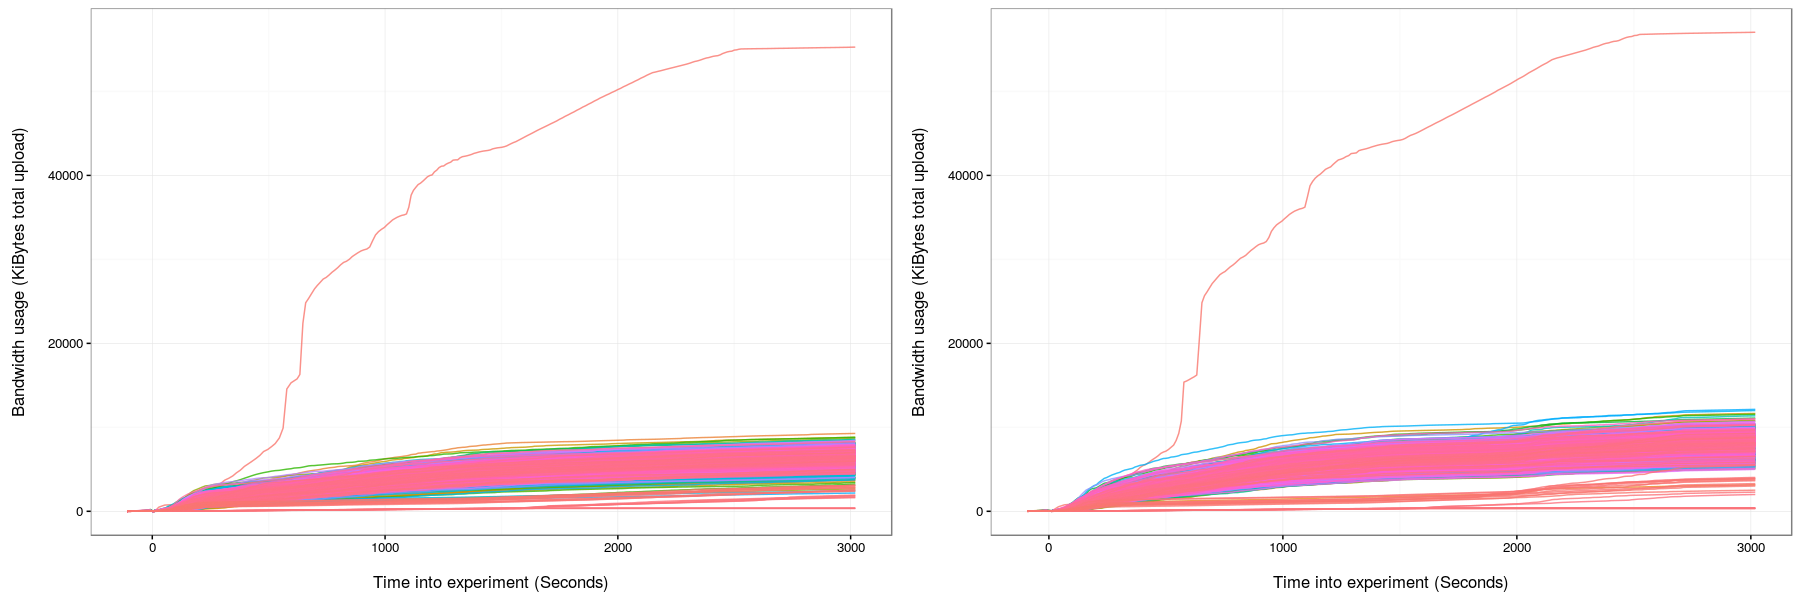
\includegraphics[width=\linewidth]{experimentation/images/send.png}}
	\caption{A side by side comparison of two \enquote{allchannel} experiment runs. Left the current code base, right asynchronous Dispersy with blocking I/O.}
	\label{fig:side_by_side_send}
\end{figure} 

Tribler has an experiment runner framework for Dispersy and Tribler: Gumby.
Using Gumby, one can specify configurations and scenario files to be executed.

Configuration files specify all the settings needed in order to run an experiment using Gumby.
Scenario file allows for a carefully timed execution of functions; each line in a scenario file specifies which node executes which function at what time. \todo{Example of such a scenario file? yes/no?}
Currently, Gumby is being used to run an experiment on the DAS5 super computer\footnote{\url{http://www.cs.vu.nl/das5/}}.
Whenever a push happens on a pull request on GitHub, our Jenkins continuous integration system automatically schedules this experiment to be run.

Using Gumby, statistics such as CPU, memory consumption and I/O are automatically tracked.
Any additional information that one wishes to track can be logged and parsed using auxiliary post experiment scripts.
Currently, graphs are being generated in the R programming language using the ggplot2 library.

To obtain a regression testing system, we decided to extend Gumby.
To obtain the data for comparison, the proposed commits first have to be run inside an experiment using a predetermined scenario and configuration file.
Once this experiment is done, Jenkins can fetch the data of the last successful experiment run of the current code base.
Next, using the data from both experiments we generate graphs.
By creating a side-by-side plot of two graphs using the same scales, developers can immediately see any changes, see Figure~\ref{fig:side_by_side_send}.\todo{Replace the right one with the dispersy async + non-block, should be more of a change.}